\section{Api rest}

\begin{flushleft}
Pour terminer cette extension, il a fallu ajouter une requête API comme illustrée dans le diagramme de séquence sur \textbf{Comparer les données de consommations}. Nous retrouvons donc une requête API nommée \textbf{List Consumption Simulation} qui appellera la méthode \textbf{getConsumptionOfSimulation}. Pour cela, nous envoyons le token ainsi que la date de départ et la date de fin. Nous recevons en retour une liste de dates et de données de consommations journalières.
\end{flushleft}

\begin{flushleft}
Notez qu'il a fallu ajouter les paramètres concernant l'extension lors de la création d'un portefeuille et que nous pouvons également envoyer en plus lors d'une requête \textbf{List Wallets} pour que le client puisse voir toutes les informations liées à celui-ci.
\end{flushleft}

\begin{figure}[h]
\centering
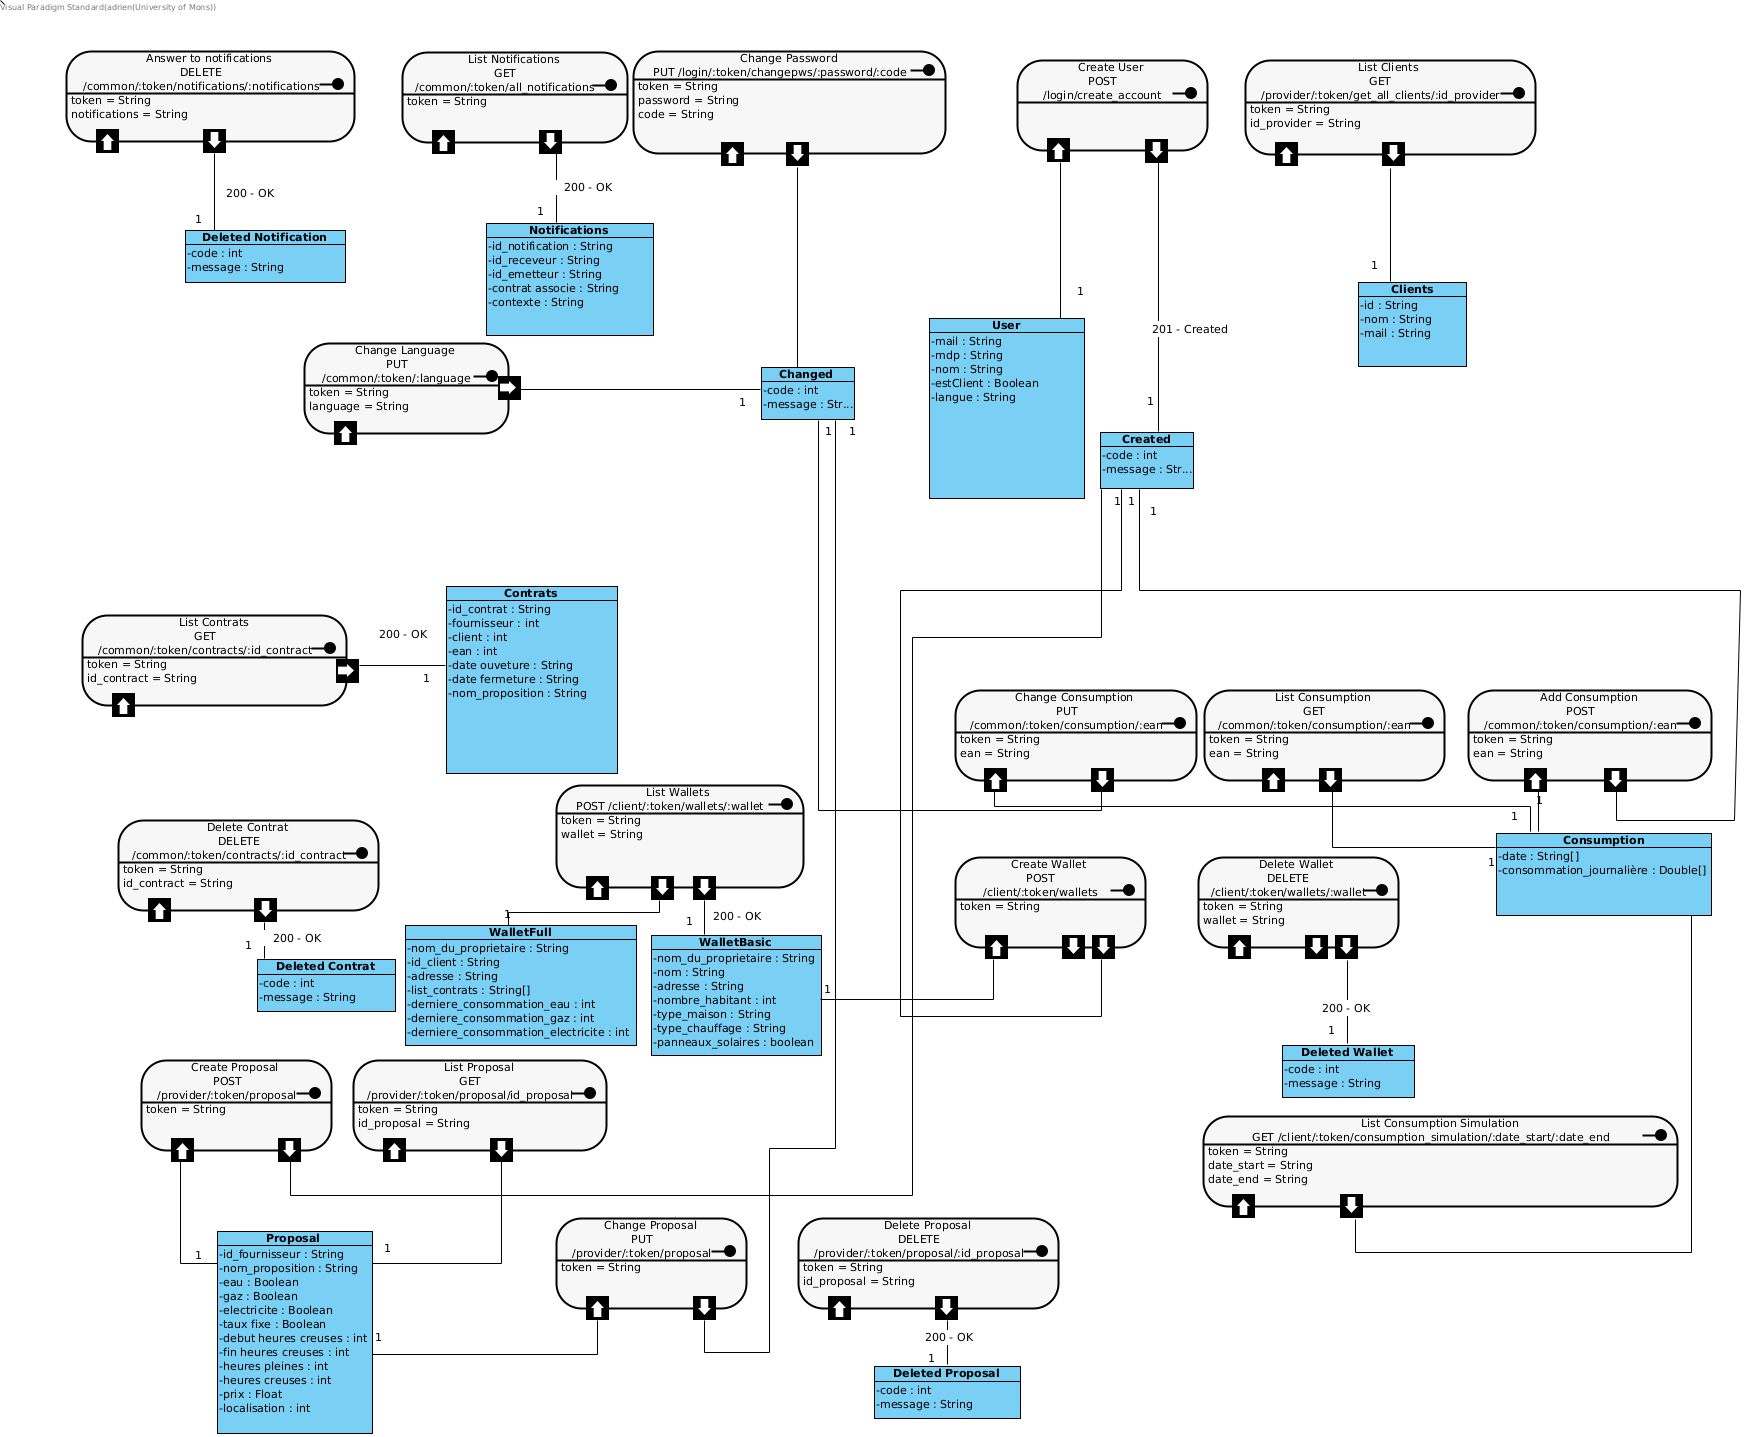
\includegraphics[width=1\textwidth]{extension-adrien/Api-rest/img/apirest.png}
\end{figure}
